\documentclass[english, xcolor = {table}]{beamer}
\usepackage{slides_style}
\usepackage{mathtools}
\usepackage{dsfont}


%\usetikzlibrary{shapes.geometric,positioning}

\newcommand{\EoL}[1][2]{\lang{Eo}\text{-}{#1}\text{-}\lang{L}}


\title[Proofs and Computations]{
    Monotone Circuit Lower Bounds from Resolution
}

\author[Sokolov D.]{
    Dmitry Sokolov\\
    KTH University\\
    \vspace{1cm}
    joint work with\\
    Ankit Garg, Mika G{\"{o}}{\"{o}}s, Pritish Kamath, Robert Robere
}  


\date{The University of Chicago\\
	January 15\\
	2019
}


\AtBeginSection[]{
    \begin{frame}
        \vfill
        \centering
        \usebeamerfont{title}\insertsectionhead\par%
        \vfill
    \end{frame}
}


\begin{document}

    \maketitle

    \section{Introduction: Proof systems}

    \section{Introduction}

\begin{frame}{Definitions}

    \begin{block}{Ensembles of distributions}
        Ensemble of distributions $\Dis = \{D_n\}_{n = 1}^{\infty}$.

        \vspace{0.15cm}
        
        $\Dis \in \Samp[n^k] \Leftrightarrow$ there is a randomized $O(n^k)$-time algorithm $A$
        such that $D_n$ and $A(1^n)$ are equally distributed.
    \end{block}

   	$\PSamp = \bigcup\limits_k \Samp[n^k]$.

	\pause
    
	\begin{block}{Heuristic computations}
		$\Lan$ is a language, $\Dis$ is an ensemble of distributions.

        \vspace{0.15cm}
        
        $(\Lan, \Dis) \in \Heur[\delta]\DTime[n^k] \Leftrightarrow$ there is $O(n^k)$-time algorithm $A$ such that
		$\Pr\limits_{x \gets D_n} [A(x) = L(x)] > 1 - \delta$.
	\end{block}

    $\HeurP[\delta] = \bigcup\limits_k \Heur[\delta]\DTime[n^k]$.
\end{frame}

\begin{frame}{``Easy'' problems}

    \begin{theorem}[Gurevich and Shelah, 1987]
        Let $\lang{HP}$ denote the language of Hamiltonian graphs. Then $(\lang{HP}, \lang{U}) \in
        \Heur[\frac{1}{2^{O(\sqrt{n})}}]\DTime[n]$. 
    \end{theorem}
    \pause
    \begin{theorem}[Babai, Erdos and Selkow, 1980]
        Let $\lang{GI}$ denote the language of pairs of isomorphic graphs. Then $(\lang{GI}, \lang{U}) \in
        \Heur[\frac{1}{\sqrt[7]{n}}]\DTime[n]$. 
    \end{theorem}
\end{frame}

    \section{Part I: Dag Protocols and Lifting}

    \newcommand{\ba}{{\color{blue} $\boldsymbol{\forall}$}}
\newcommand{\be}{{\color{blue} $\boldsymbol{\exists}$}}

\begin{frame}{Следствия}
    $m = n^{O(1)}$, $w(\varphi)$~--- минимальная ширина резолюционного доказательства $\varphi$.

    \pause
    \begin{enumerate}
        \item \ba $\varphi$ число строк в $\CP$-доказательстве $\varphi \circ \Ind_m$ не менее
            $n^{w(\varphi)}$.
        \pause
        \item \textbf{($\CP$ vs. $\NS$)} \be $\varphi$, что:
            \begin{itemize}
                \item над любым полем $\mathbb{F}$ формула $\varphi$ имеет
                    $\NS_{\mathbb{F}}$-доказательство степени $O(\log(n))$;
                \item любое $\CP$-доказательство $\varphi$ имеет размер не менее $2^{n^{\varepsilon}}$,
                    где $\varepsilon > 0$.
            \end{itemize}
        \pause
        \vspace{0.2cm}
        \item \be $f$, которая может быть посчитана при помощи $mSP$ размера $\poly(n)$ над любым полем,
            но любая монотонная вещественная схема для $f$ имеет размер не менее $2^{n^{\varepsilon}}$,
            где $\varepsilon > 0$.
        \pause
        \item \be $f \in \NC^2$, что любая монотонная вещественная схема для $f$ имеет размер не менее
            $2^{n^{\varepsilon}}$, где $\varepsilon > 0$.
    \end{enumerate}
\end{frame}

    \begin{frame}{Tree-like communication protocols. $S \subseteq X \times Y \times \mathcal{T}$}

    Alice receives $x \in X$ and Bob receives $y \in Y$. A communication protocols corresponds to a tree:

    \begin{columns}[t]
		\begin{column}{0.6\textwidth}
            \begin{itemize}
                \item<2-> inner vertices are marked by players;
	            \item<3-> if current player sends a bit they move to next vertex;
    		    \item<8-> leaves are marked by answers.
	        \end{itemize}

            \vspace{0.5cm}
    		\onslide<9->{
                Reformulation: at each node players try to answer for the question: ``Which vertex will
                be next?''
            }
        \end{column}
        
		\begin{column}{0.3\textwidth}
            \tikzstyle{inner} = [thin, circle, minimum size = 0.3cm, draw, inner sep = 0.1pt, black]
\tikzstyle{inner_g} = [thin, circle, minimum size = 0.3cm, draw, inner sep = 0.1pt, black, fill = green]
\tikzstyle{inner_r} = [thin, circle, minimum size = 0.3cm, draw, inner sep = 0.1pt, black, fill = red]
\tikzstyle{inner_b} = [thin, circle, minimum size = 0.3cm, draw, inner sep = 0.1pt, black, fill = blue!50!white]
\tikzstyle{ed} = [thick, ->, draw, black]

    
\begin{tikzpicture}
    \only<-3, 5->{
        \node[inner] (a) at (0, 0) {\scriptsize $a$};
	}
    \only<4>{
        \node[inner_g] (a) at (0, 0) {\scriptsize $a$};
    }

    \only<-4, 6->{
        \node[inner] (b) at (-0.9, -1.2) {\scriptsize $b$};
	}
    \only<5>{
        \node[inner_g] (b) at (-0.9, -1.2) {\scriptsize $b$};
    }

    \node[inner] (c) at (0.9, -1.2) {\scriptsize $a$};
    \node[inner, label = below:$t_1$] (d) at (-1.5, -2.4) {};

    \only<-5, 7->{
        \node[inner] (e) at (-0.3, -2.4) {\scriptsize $b$};
	}
    \only<6>{
        \node[inner_g] (e) at (-0.3, -2.4) {\scriptsize $b$};
    }

    \node[inner] (e2) at (0.3, -2.4) {\scriptsize $b$};
    \node[inner, label = below:$t_4$] (f) at (1.5, -2.4) {};

    \only<-6, 9->{
        \node[inner, label = below:$t_2$] (g) at (-1.5, -4.3) {};
	}
    \only<7-8>{
        \node[inner_g, label = below:$t_2$] (g) at (-1.5, -4.3) {};
    }
    
    \node[inner, label = below:$t_3$] (h) at (-0.25, -4.3) {};
	\node[inner, label = below:$t_3$] (g2) at (1.5, -4.3) {};
    \node[inner, label = below:$t_2$] (h2) at (0.25, -4.3) {};
    
    \path (a) edge[ed] (b);
    \path (a) edge[ed] (c);
    \path (b) edge[ed] (d);
    \path (b) edge[ed] (e);
    \path (c) edge[ed] (e2);
    \path (c) edge[ed] (f);
    \path (e) edge[ed] (g);
    \path (e) edge[ed] (h);
    \path (e2) edge[ed] (g2);
    \path (e2) edge[ed] (h2);
\end{tikzpicture}

		\end{column}
	\end{columns}

\end{frame}


\begin{frame}{Tree vs. Dag}

	\begin{columns}[t]
		\begin{column}{0.52\textwidth}
            \begin{center}
                Tree-like world.
                \only<1-2>{
                    ``Which vertex will be next?''
                }
                \only<3->{
                    \alert{``Are we in good vertex?''}
                }
                \vspace{0.2cm}
                \tikzstyle{inner} = [thin, circle, minimum size = 0.3cm, draw, inner sep = 0.1pt, black]
\tikzstyle{inner_g} = [thin, circle, minimum size = 0.3cm, draw, inner sep = 0.1pt, black, fill = green]
\tikzstyle{ed} = [thick, ->, draw, black]

    
\begin{tikzpicture}[>=stealth']
    \node[inner_g] (a) at (0, 0) {};
    \node[inner_g] (b) at (-0.9, -1.2) {};
    \node[inner] (c) at (0.9, -1.2) {};
    \node[inner] (d) at (-1.5, -2.4) {};
    \node[inner_g] (e) at (-0.3, -2.4) {};
    \node[inner] (e2) at (0.3, -2.4) {};
    \node[inner] (d) at (-1.5, -2.4) {\scriptsize $t_1$};
    \node[inner_g] (e) at (-0.3, -2.4) {};
    \node[inner] (e2) at (0.3, -2.4) {};
    \node[inner] (f) at (1.5, -2.4) {\scriptsize $t_4$};
    \node[inner_g] (g) at (-1.5, -4.3) {\scriptsize $t_2$};
    \node[inner] (h) at (-0.25, -4.3) {\scriptsize $t_3$};
	\node[inner] (g2) at (1.5, -4.3) {\scriptsize $t_3$};
    \node[inner] (h2) at (0.25, -4.3) {\scriptsize $t_2$};
    
    \path (a) edge[ed] (b);
    \path (a) edge[ed] (c);
    \path (b) edge[ed] (d);
    \path (b) edge[ed] (e);
    \path (c) edge[ed] (e2);
    \path (c) edge[ed] (f);
    \path (e) edge[ed] (g);
    \path (e) edge[ed] (h);
    \path (e2) edge[ed] (g2);
    \path (e2) edge[ed] (h2);
\end{tikzpicture}

            \end{center}
        \end{column}

        \pause
		\begin{column}{0.48\textwidth}
            \begin{center}
                Dag-like world. ``Are we in good vertex?''
                \vspace{0.2cm}
                \only<1>{
	\tikzstyle{inner} = [thin, circle, minimum size = 0.3cm, draw, inner sep = 0.1pt, black, opacity = 0]
	\tikzstyle{inner_g} = [thin, circle, minimum size = 0.3cm, draw, inner sep = 0.1pt, black, fill =
	    green, opacity = 0]
	\tikzstyle{ed} = [thick, ->, draw, black, opacity = 0]
}
\only<2->{
	\tikzstyle{inner} = [thin, circle, minimum size = 0.3cm, draw, inner sep = 0.1pt, black, opacity = 1]
	\tikzstyle{inner_g} = [thin, circle, minimum size = 0.3cm, draw, inner sep = 0.1pt, black, fill =
	    green, opacity = 1]
	\tikzstyle{ed} = [thick, ->, draw, black, opacity = 1]
}

    
\begin{tikzpicture}[>=stealth']
    \node[inner_g] (a) at (0, 0) {};
    \node[inner_g] (b) at (-0.9, -1.2) {};
    \node[inner] (c) at (0.9, -1.2) {};
    \node[inner] (d) at (-1.5, -2.4) {\scriptsize $t_1$};
    \node[inner_g] (e) at (-0.3, -2.4) {};
    \node[inner_g] (f) at (1, -2.4) {};
    \node[inner_g] (g) at (-1.5, -4.3) {\scriptsize $t_2$};
    \node[inner] (h) at (-0.25, -4.3) {\scriptsize $t_3$};
	\node[inner_g] (g2) at (1.5, -4.3) {\scriptsize $t_3$};
    \node[inner] (h2) at (0.25, -4.3) {\scriptsize $t_2$};
    
    \path (a) edge[ed] (b);
    \path (a) edge[ed] (c);
    \path (b) edge[ed] (d);
    \path (b) edge[ed] (e);
    \path (c) edge[ed] (e);
    \path (c) edge[ed] (f);
    \path (e) edge[ed] (g);
    \path (e) edge[ed] (h);
    \path (f) edge[ed] (g2);
    \path (f) edge[ed] (h2);
\end{tikzpicture}

            \end{center}
		\end{column}
	\end{columns}

    \pause
    \pause
    \vspace{0.4cm}
    Alice and Bob independently answer for this question.
\end{frame}

\begin{frame}{Dag protocols}
    \vspace{-0.8cm}
    \begin{columns}[t]
        \begin{column}{0.58\textwidth}
            \begin{itemize}
                \item $H$ is a graph with out degree $2$, $\forall h \in H, ~ C_h \subseteq X \times Y$;
                \item $C_{root} = X \times Y$;
                \item $a, b$ are children of $h$ $\Rightarrow$ $C_{h} \subseteq C_{a} \cup C_{b}$;
                \item $h$ is a leaf $\Rightarrow$ $h$ is marked by common solution for $C_h$.
            \end{itemize}
        \end{column}

		\begin{column}{0.38\textwidth}
            \begin{center}
                \tikzstyle{inner} = [thin, circle, minimum size = 0.3cm, draw, inner sep = 0.1pt, black, opacity = 1]
\tikzstyle{inner_g} = [thin, circle, minimum size = 0.3cm, draw, inner sep = 0.1pt, black, fill =
    green, opacity = 1]
\tikzstyle{ed} = [thick, ->, draw, black, opacity = 1]

    
\begin{tikzpicture}[>=stealth']
    \node[inner_g] (a) at (0, 0) {};
    \node[inner_g] (b) at (-0.9, -0.7) {};
    \node[inner] (c) at (0.9, -0.7) {};
    \node[inner] (d) at (-1.5, -1.6) {\scriptsize $t_1$};
    \node[inner_g] (e) at (-0.3, -1.6) {};
    \node[inner_g] (f) at (1, -2) {};
    \node[inner_g] (g) at (-1.5, -3) {\scriptsize $t_2$};
    \node[inner] (h) at (-0.25, -3) {\scriptsize $t_3$};
    \node[inner_g] (g2) at (1.5, -3) {\scriptsize $t_3$};
    \node[inner] (h2) at (0.25, -3) {\scriptsize $t_2$};
    
    \path (a) edge[ed] (b);
    \path (a) edge[ed] (c);
    \path (b) edge[ed] (d);
    \path (b) edge[ed] (e);
    \path (c) edge[ed] (e);
    \path (c) edge[ed] (f);
    \path (e) edge[ed] (g);
    \path (e) edge[ed] (h);
    \path (f) edge[ed] (g2);
    \path (f) edge[ed] (h2);
\end{tikzpicture}

            \end{center}
		\end{column}
	\end{columns}

    \pause
    \begin{columns}[t]
		\begin{column}{0.48\textwidth}
            \begin{center}
                Rectangle (boolean) dag:
                \vspace{0.2cm}
                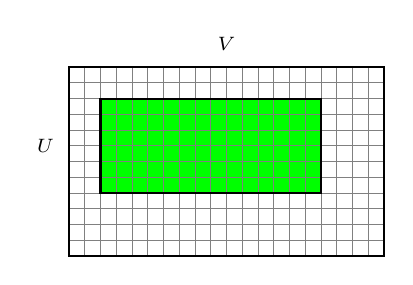
\begin{tikzpicture}
    \draw[fill = green] (0.4, -0.4) rectangle (3.2, -1.6);
    \draw[step = 0.2, gray, thin] (0, 0) grid (4, -2.4);
    \draw[black, thick] (0, 0) rectangle (4, -2.4);
    \draw[black, thick] (0.4, -0.4) rectangle (3.2, -1.6);
    \node at (-0.3, -1.) {\scriptsize $U$};
    \node at (2, 0.3) {\scriptsize $V$};
\end{tikzpicture}

            \end{center}
        \end{column}

		\begin{column}{0.48\textwidth}
            \begin{center}
                Triangle (real) dag:
                \vspace{0.2cm}
                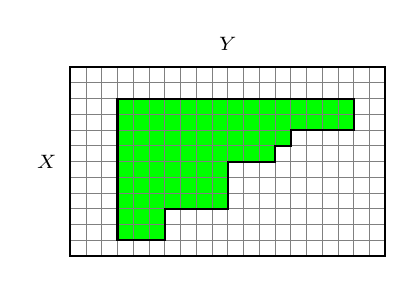
\begin{tikzpicture}
    \draw[fill = green] (0.6, -0.4) -- (3.6, -0.4) -- (3.6, -0.8) -- (2.8, -0.8) -- (2.8, -1) --
    	(2.6, -1) -- (2.6, -1.2) -- (2, -1.2) -- (2, -1.8) -- (1.2, -1.8) -- (1.2, -2.2) -- (0.6, -2.2) --
        cycle;
    \draw[step = 0.2, gray, thin] (0, 0) grid (4, -2.4);
    \draw[black, thick] (0.6, -0.4) -- (3.6, -0.4) -- (3.6, -0.8) -- (2.8, -0.8) -- (2.8, -1) --
    	(2.6, -1) -- (2.6, -1.2) -- (2, -1.2) -- (2, -1.8) -- (1.2, -1.8) -- (1.2, -2.2) -- (0.6, -2.2) --
        cycle;
    \draw[black, thick] (0, 0) rectangle (4, -2.4);
    \node at (-0.3, -1.2) {\scriptsize $X$};
    \node at (2, 0.3) {\scriptsize $Y$};
\end{tikzpicture}

            \end{center}
		\end{column}
	\end{columns}
\end{frame}


\begin{frame}{$\KWm$ relation (Karchmer, Wigderson 1990)}

    $f\colon \{0, 1\}^n \to \{0, 1\}$ is a monotone partial function
    
    \begin{itemize}
        \item Alice receives $x \in f^{-1}(1)$, Bob receives $y \in f^{-1}(0)$;
        \item goal is to find $i$ such that $x_i = 1 \land y_i = 0$.
    \end{itemize}

    \pause

    \begin{theorem}[Razborov 95; Pudl{\'{a}}k 10; S 17]
        Monotone boolean circuit for $f$ of size $S$ $\Leftrightarrow$ rectangle dag protocol of size $S$
        for the $\KWm[f]$ relation.
    \end{theorem}

    \pause

    \begin{theorem}[Hrube{\v{s}} Pudl{\'{a}}k 17]
        Monotone real circuit for $f$ of size $S$ $\Leftrightarrow$ triangle dag protocol of size $S$
        for the $\KWm[f]$ relation.
    \end{theorem}
\end{frame}


\begin{frame}{Canonical search problem $\Search_{\varphi}$ (Lov{\'{a}}sz et al. 1994)}
    
    $\varphi(x, y)$ is an unsatisfiable CNF formula:
    \begin{itemize}
        \item Alice receives an assignment to the variables $x$, Bob receives an assignment to the
            variables $y$;
        \item goal is to find a clause $C \in \varphi$ that is unsatisfied by this assignment.
    \end{itemize}

    \pause

    \begin{theorem}[Kraj{\'{\i}}{\v{c}}ek 95; S 17]
        $CC_{\log(n)}$ proof of $\varphi$ of size $S$ $\Rightarrow$ rectangle dag protocol for
        $\Search_{\varphi}$ of size $\poly(n) S$.
    \end{theorem}

    Resolution, $\CP^*$, $\dots$ are $CC_{\log(n)}$ proof systems.

    \pause
    
    \begin{theorem}[S 17]
        $\CP$ of $\varphi$ of size $S$ $\Rightarrow$ triangle dag protocol for $\Search_{\varphi}$ of
        size $S$.
    \end{theorem}
\end{frame}
    \begin{frame}{Decision dag (conjunction dag). $S \subseteq \{0, 1\}^n \times \mathcal{T}$}
    $C(\rho) = \{z \in \{0, 1\}^n \mid z \sim \rho\}$
    
    \begin{columns}[t]
        \begin{column}{0.55\textwidth}
            \begin{itemize}
                \item $H$ is a graph with out degree $2$, $\forall h \in H, ~ {\rho}_h$ is a partial
                    assignment;
                \item $\rho_{root} = \emptyset$ ($C(\rho_{root}) \equiv 1$);
                \item $a, b$ are children of $h$ $\Rightarrow$ $C(\rho_{h}) \subseteq C(\rho_a) \cup
                    C(\rho_b)$;
                \item $h$ is a leaf $\Rightarrow$ $h$ is marked by common solution for $C(\rho_h)$.
            \end{itemize}
        \end{column}

		\begin{column}{0.4\textwidth}
            \begin{center}
                \tikzstyle{inner} = [thin, circle, minimum size = 0.4cm, draw, inner sep = 0.1pt, black, opacity = 1]
\tikzstyle{inner_g} = [thin, circle, minimum size = 0.4cm, draw, inner sep = 0.1pt, black, fill =
    green, opacity = 1]
\tikzstyle{ed} = [thick, ->, draw, black, opacity = 1]

    
\begin{tikzpicture}
    \node[inner_g] (a) at (0, 0) {};
    \node[inner_g] (b) at (-0.9, -1.2) {};
    \node[inner] (c) at (0.9, -1.2) {\scriptsize $\rho_h$};
    \node[inner] (d) at (-1.5, -2.4) {\scriptsize $t_1$};
    \node[inner_g] (e) at (-0.3, -2.4) {\scriptsize $\rho_a$};
    \node[inner_g] (f) at (1, -2.4) {\scriptsize $\rho_b$};
    \node[inner_g] (g) at (-1.5, -4.3) {\scriptsize $t_2$};
    \node[inner] (h) at (-0.25, -4.3) {\scriptsize $t_3$};
	\node[inner_g] (g2) at (1.5, -4.3) {\scriptsize $t_3$};
    \node[inner] (h2) at (0.25, -4.3) {\scriptsize $t_2$};
    
    \path (a) edge[ed] (b);
    \path (a) edge[ed] (c);
    \path (b) edge[ed] (d);
    \path (b) edge[ed] (e);
    \path (c) edge[ed] (e);
    \path (c) edge[ed] (f);
    \path (e) edge[ed] (g);
    \path (e) edge[ed] (h);
    \path (f) edge[ed] (g2);
    \path (f) edge[ed] (h2);
\end{tikzpicture}

            \end{center}
		\end{column}
	\end{columns}

    Width of decision dag is $\max\limits_{h \in H} |\rho_h|$.
\end{frame}

\begin{frame}{Result}
    \begin{itemize}
        \item $S \subseteq \{0, 1\}^n \times \mathcal{T}$;
        \item $w(S)$ the least width of decision dag;
        \pause
        \item $\Ind: [m] \times \{0, 1\}^m \to \{0, 1\}$, where $m = n^{O(1)}$;
        \item $\Ind(x, y) = y_x$;
        \pause
        \item $S \circ \Ind$ is composed search problem.
    \end{itemize}

    \only<1-3>{
    \onslide<3>{
        \begin{center}
              \begin{tikzpicture}
    \node[thick, circle, draw] (S) at (0, 0) {\Large $S$};
    
    \foreach \i in {1, 2, ..., 5}{
        \node (z\i) at (-3 + \i, -1.5) {$z_{\i}$};
        \draw[->] (z\i) -- (S);
    }
    
    \node[minimum height = 1cm, single arrow, draw] at (3, 0) {composition};

    \node[thick, circle, draw] (S1) at (6, 0) {\Large $S$};

    \foreach \i in {1, 2, ..., 5}{
        \node[draw, circle] (i\i) at (3 + \i, -1.5) {\scriptsize $g$};
        \draw[->] (i\i) -- (S1);

        \node (x\i) at (2.75 + \i, -2.4) {\scriptsize $x_{\i}$};
        \node (y\i) at (3.25 + \i, -2.4) {\scriptsize $y_{\i}$};
        \draw[->] (x\i) -- (i\i);
        \draw[->] (y\i) -- (i\i);
    }
\end{tikzpicture}
        \end{center}
    }}

    \only<4>{
        \vspace{0.86cm}
        \begin{theorem}
            Rectangle (triangle) dag complexity of $S \circ \Ind_m$ is $n^{\theta(w(S))}$.  
        \end{theorem}
        \vspace{1.8cm}
    }
\end{frame}
    \begin{frame}{Open problems}

    \begin{itemize}
        \item Lower bounds for $\EQ$ dag protocols.
        \item Lower bounds for randomized dag protocols.
        \item Lower bounds NOF model of dag protocols.
        \item Can we prove the same result for constant size gadget?
    \end{itemize}

    \begin{block}{Conjecture}
        Randomized rectangle dag complexity of $S \circ \Ind_{m}$ is $n^{\Theta(w'(S))}$, where $w'(S)$ is
        width of ``random resolution refutation'' of $S$.
    \end{block}
\end{frame}

    \section{Part II: From Proofs to Computations}

    \begin{frame}{Certificate of unsatisfiability}

    $\varphi(x, y) = \bigwedge\limits_{i = 1}^{m} C_i(x, y)$

    \vspace{0.5cm}

    $U_{\varphi}, V_{\varphi} \subseteq \{0, 1\}^m$:
    \begin{itemize}
        \item $A \in U_{\varphi} \Leftrightarrow \bigwedge\limits_{i \in A} C_i|_{x}$ is satisfiable;
        \item $A \in V_{\varphi} \Leftrightarrow \bigwedge\limits_{i \in A} C_i|_{y}$ is unsatisfiable.
    \end{itemize}

    $C_{x}$ ($C_{y}$) is a restriction of $C$ to the variables from $x$ ($y$) part.

    \begin{lemma}[Hrube{\v{s}}, Pudl{\'{a}}k 17 (implicit)]
        $\Search_{\varphi} \approx \KWm(U_{\varphi}, V_{\varphi})$.
    \end{lemma}
\end{frame}


\begin{frame}{Monotone span programs over field $\mathbb{F}$ (Karchmer, Wigderson 93)}

    \only<1>{
        \begin{center}
            \begin{tabular}{|c|cccccccc|}
                \hline
                $x_1$ & 0 & 2 & 3 & 1 & 0 & 2 & 1 & 0\\
                $x_3$ & 2 & 1 & 0 & 0 & 2 & 0 & 0 & 1\\
                $x_4$ & 1 & 0 & 0 & 0 & 0 & 0 & 0 & 0\\
                $x_5$ & 3 & 2 & 1 & 4 & 0 & 2 & 1 & 0\\
                $x_1$ & 0 & 2 & 3 & 1 & 3 & 2 & 4 & 0\\
                \hline
            \end{tabular}
        \end{center}
    }
      
	\only<2->{
        \begin{minipage}{0.5\linewidth}
            \def\firstrow{
            	$x_1$ & 1 & 0 & 1\\
                $x_1$ & 1 & 0 & 1\\
            }
            \only<5-6>{
                \def\firstrow{
            	    \rowcolor{green!40}[1.001\tabcolsep][1.001\tabcolsep] $x_1$ & 1 & 0 & 1\\
                    \rowcolor{green!40}[1.001\tabcolsep][1.001\tabcolsep] $x_1$ & 1 & 0 & 1\\
                }
            }

            \def\secondrow{
                $x_2$ & 0 & 1 & 1 \\
                $x_2$ & 1 & 1 & 0 \\
            }
            \only<8-9>{
                \def\secondrow{
            	    \rowcolor{red!40}[1.001\tabcolsep][1.001\tabcolsep] $x_2$ & 0 & 1 & 1 \\
                    \rowcolor{red!40}[1.001\tabcolsep][1.001\tabcolsep] $x_2$ & 1 & 1 & 0 \\
                }
            }

            \def\thirdrow{
                $x_3$ & 0 & 1 & 1 \\
                $x_3$ & 1 & 0 & 1 \\
            }
            \only<5-6>{
                \def\thirdrow{
            	    \rowcolor{green!40}[1.001\tabcolsep][1.001\tabcolsep] $x_3$ & 0 & 1 & 1 \\
                    \rowcolor{green!40}[1.001\tabcolsep][1.001\tabcolsep] $x_3$ & 1 & 0 & 1 \\
                }
            }
              
            \begin{center}
                \begin{tabular}{|c|ccc|}
                    \hline
                    \firstrow
                    \secondrow
                    \thirdrow
                    \hline
                \end{tabular}
            \end{center}
        \end{minipage}%
        \begin{minipage}{0.5\linewidth}
            \pause
            \pause
            \begin{itemize}
                \item Is there $(1, 1, 1, \dots)$ in the span of selected vectors?
                \pause  
                \item $f(1, 0, 1) = \only<4-5>{~?} \only<6->{1;}$
                \pause
                \pause
                \pause
                \item $f(0, 1, 0) = \only<7-8>{~?} \only<9->{0;}$
                \pause
                \pause
                \pause
                \item $MAJ(x_1, x_2, x_3)$.
            \end{itemize}
        \end{minipage}
    }
    
    \vspace{0.15cm}

    \pause
    Size of the program is the number of columns.

    \pause
    \vspace{0.3cm}

    \begin{minipage}{0.5\linewidth}
        \begin{center}
        	AND
            
            \begin{tabular}{|c|cc|}
                \hline
                $x_1$ & 1 & 0\\
                $x_2$ & 0 & 1\\
                \hline
            \end{tabular}
        \end{center}
    \end{minipage}%
    \begin{minipage}{0.5\linewidth}
        \begin{center}
        	OR
            
            \begin{tabular}{|c|c|}
                \hline
                $x_1$ & 1\\
                $x_2$ & 1\\
                \hline
            \end{tabular}
        \end{center}
    \end{minipage}

    \pause
    \begin{lemma}[Pudl{\'{a}}k, Sgall 98]
        $\forall f, mSP(f) \le mF(f)$.
    \end{lemma}
\end{frame}


\begin{frame}{Span programs and Nullstellensatz}

    \begin{lemma}[modification of Pudl{\'{a}}k, Sgall 98]
        $\NS$-proof of $\varphi(x, y)$ of $y$-degree $d$ $\Rightarrow$ $mSP(U_{\varphi}, V_{\varphi})$ of
        size $n^d$.
    \end{lemma}

    \pause

    \begin{lemma}[Pitassi, Robere 18]
        There is gadget $g$ such that $mSP(U_{\varphi \circ g}, V_{\varphi \circ g}) =
        n^{\Theta(\NS(\varphi))}$.
    \end{lemma}

    \pause

    \begin{lemma}
        $\NS$-proof of $\varphi$ of degree $d$ $\Rightarrow$ $\NS$-proof of $\varphi \circ \Ind_m$ of
        $y$-degree $d$.
    \end{lemma}

    $\Ind_m(x, y) = \sum\limits_{s \in [m]} \mathds{1}_{x = s} \cdot y_s$
\end{frame}


\begin{frame}{Separations}

    \begin{center}
        $\varphi$ is unsat CNF
	\end{center}

    \begin{minipage}{0.5 \textwidth}
        \centering
        Upper bound
    \end{minipage}%
    \begin{minipage}{0.5 \textwidth}
        \centering
        Lower bound
    \end{minipage}

    \pause
    \vspace{0.4cm}

    \begin{minipage}{0.5 \textwidth}
        \centering
        $\NS$-degree of $\varphi$
    \end{minipage}%
    \begin{minipage}{0.5 \textwidth}
        \centering
        resolution width of $\varphi$
    \end{minipage}

    \pause
    \vspace{0.3cm}

    \begin{minipage}{0.5 \textwidth}
        \centering
        $\Downarrow$ [PS]

        \vspace{0.3cm}

        $mSP(U_{\varphi \circ \Ind}, V_{\varphi \circ \Ind})$
    \end{minipage}%
    \begin{minipage}{0.5 \textwidth}
        \centering
        $\Downarrow$

        \vspace{0.3cm}
        
        $mRC(U_{\varphi \circ \Ind}, V_{\varphi \circ \Ind})$
    \end{minipage}


    \pause
    \vspace{1cm}
    Goal is to find any formula of small width that separates Nullstellensatz and Resolution.

\end{frame}
    \begin{frame}{Span programs and Nullstellensatz}

    \begin{lemma}[modification of Pudl{\'{a}}k, Sgall 98]
        $\NS$-proof of $\varphi(x, y)$ of $y$-degree $d$ $\Rightarrow$ $mSP(U_{\varphi}, V_{\varphi})$ of
        size $n^d$.
    \end{lemma}

    \pause

    \begin{lemma}[Pitassi, Robere 18]
        There is gadget $g$ such that $mSP(U_{\varphi \circ g}, V_{\varphi \circ g}) =
        n^{\Theta(\NS(\varphi))}$.
    \end{lemma}

    \pause

    \begin{lemma}
        $\NS$-proof of $\varphi$ of degree $d$ $\Rightarrow$ $\NS$-proof of $\varphi \circ \Ind_m$ of
        $y$-degree $d$.
    \end{lemma}

    $\Ind_m(x, y) = \sum\limits_{s \in [m]} \mathds{1}_{x = s} \cdot y_s$
\end{frame}


\begin{frame}{Separations}

    \begin{center}
        $\varphi$ is unsat CNF
	\end{center}

    \begin{minipage}{0.5 \textwidth}
        \centering
        Upper bound
    \end{minipage}%
    \begin{minipage}{0.5 \textwidth}
        \centering
        Lower bound
    \end{minipage}

    \pause
    \vspace{0.4cm}

    \begin{minipage}{0.5 \textwidth}
        \centering
        $\NS$-degree of $\varphi$
    \end{minipage}%
    \begin{minipage}{0.5 \textwidth}
        \centering
        resolution width of $\varphi$
    \end{minipage}

    \pause
    \vspace{0.3cm}

    \begin{minipage}{0.5 \textwidth}
        \centering
        $\Downarrow$ [PS]

        \vspace{0.3cm}

        $mSP(U_{\varphi \circ \Ind}, V_{\varphi \circ \Ind})$
    \end{minipage}%
    \begin{minipage}{0.5 \textwidth}
        \centering
        $\Downarrow$

        \vspace{0.3cm}
        
        $mRC(U_{\varphi \circ \Ind}, V_{\varphi \circ \Ind})$
    \end{minipage}


    \pause
    \vspace{1cm}
    Goal is to find any formula of small width that separates Nullstellensatz and Resolution.

\end{frame}
    \begin{frame}{$\EoL[k]$}
    \begin{minipage}{0.5 \linewidth}
        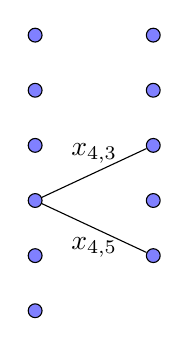
\begin{tikzpicture}[>=latex]

    \foreach \i in {1, 2, ..., 6}{
        \node[draw, circle, fill = blue!50, inner sep = 0pt, minimum size = 5pt]
            (a\i) at (0, -0.7 * \i) {};
    }

    \foreach \i in {1, 2, ..., 5}{
        \node[draw, circle, fill = blue!50, inner sep = 0pt, minimum size = 5pt]
            (b\i) at (1.5, -0.7 * \i) {};
    }
    
    \draw (a4) -- (b3) node[midway, above] {$x_{4, 3}$};
    \draw (a4) -- (b5) node[midway, below] {$x_{4, 5}$};
\end{tikzpicture}
    \end{minipage}%
    \begin{minipage}{0.5 \linewidth}
        \pause
        \pause
        \begin{itemize}
            \item $v: ~ \sum\limits_{e \in E^{in}_v} x_{e} - \sum\limits_{e \in E^{out}_v} x_{e} = c(v)$
                \textcolor{red}{$(\mathbb{R})$};
            \item $\sum\limits_{v} c(v) = k$ \textcolor{red}{$(\mathbb{R})$};
            \item $k \neq 0 \Rightarrow \EoL[k]$ is unsat. 
        \end{itemize}
    \end{minipage}

    \pause
    \begin{lemma}
        $\EoL[1]$ has a low degree $\NS$-proof over any field.
    \end{lemma}
\end{frame}

\begin{frame}{Mystery of lines}

    \begin{lemma}[1]
        \begin{itemize}
            \item $\EoL[1]$ has a low degree $\NS$-proof over any field;
            \item $\forall k, \EoL[k]$ has a low degree $\NS$-proof over $\mathbb{R}$.
        \end{itemize}
    \end{lemma}

    \begin{lemma}[2]
        $G$ is $(n, d, \alpha)$-expander $\Rightarrow$ $w(\EoL[1]) = \Omega(n)$.
    \end{lemma}

    \begin{lemma}[3]
        $k = \mathrm{char}(\mathbb{F})^{\ell} \Rightarrow \exists G$, there is no $2^{\ell} =
        \Omega(\sqrt{n})$ degree $\NS$-proof of $\EoL[k]$ over $\mathbb{F}$.
    \end{lemma}

    \begin{itemize}
        \item $(1), (2) \Rightarrow$ separation between $mSP$ and monotone circuits;
        \item $(1), (3) \Rightarrow$ $mSP$ over $\mathbb{R}$ can be stronger than $mSP$ over fields with
            $\mathrm{char} > 0$. 
    \end{itemize}

\end{frame}


\begin{frame}{Open problems}

    \begin{enumerate}
        \item $k = \mathrm{char}(\mathbb{F})^{\ell}$. Can we prove $\Omega(n)$-degree lower bound?
        \item $k = \mathrm{char}(\mathbb{F})^{\ell}$. Polynomial calculus lower bounds?
        \item Model that can capture $mSP$ and monotone circuits simultaneously?
    \end{enumerate}
\end{frame}
\end{document}

